\section{Quickstart}\label{sec:quickstart}
%
Start the QtCreator from the fresh installed SDK.

``The SDK comes with a handy SailfishOS application template that gives you a quick way to create your very first Sailfish OS application.
Just go to File-> New File or Project in the IDE''\cite{sailfishos2}
%
\begin{figure}[H]
  \centering
  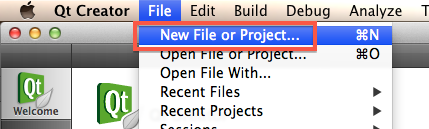
\includegraphics[scale=0.6]{../media/gfx/QtCreator/newsailfishproject01.png} 
  \caption{First example, step 1.}
  \label{fig:newsailfishproject01}
\end{figure}
%
%
\begin{figure}[H]
  \centering
  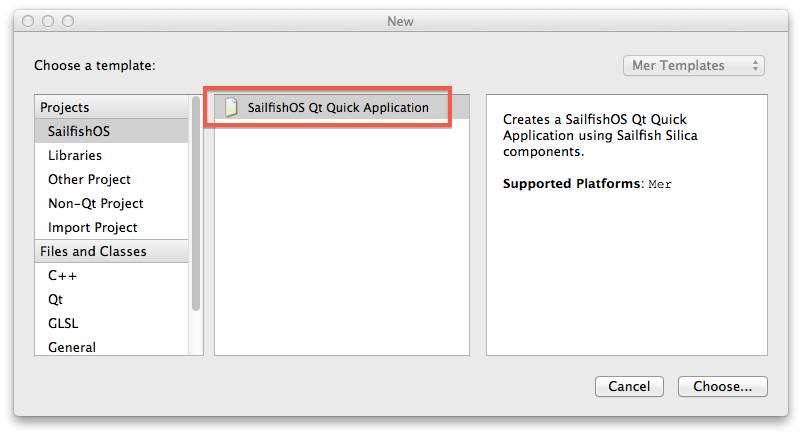
\includegraphics[scale=0.45]{../media/gfx/QtCreator/newsailfishproject02.png} 
  \caption{First example, step 2.}
  \label{fig:newsailfishproject02}
\end{figure}
%
%
\begin{figure}[H]
  \centering
  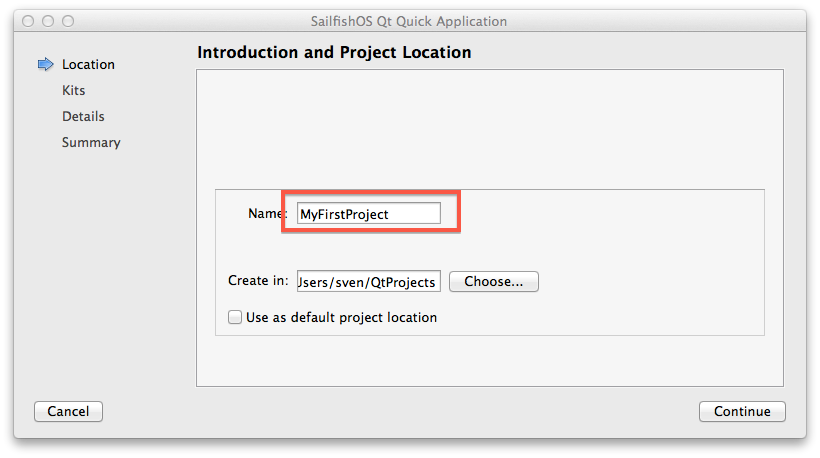
\includegraphics[scale=0.45]{../media/gfx/QtCreator/newsailfishproject03.png} 
  \caption{First example, step 3.}
  \label{fig:newsailfishproject03}
\end{figure}
%
%
\begin{figure}[H]
  \centering
  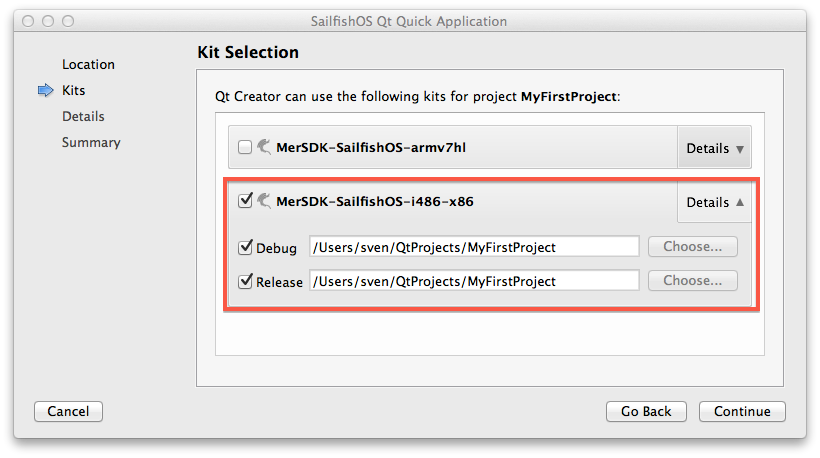
\includegraphics[scale=0.45]{../media/gfx/QtCreator/newsailfishproject04.png} 
  \caption{First example, step 4.}
  \label{fig:newsailfishproject04}
\end{figure}
%
%
\begin{figure}[H]
  \centering
  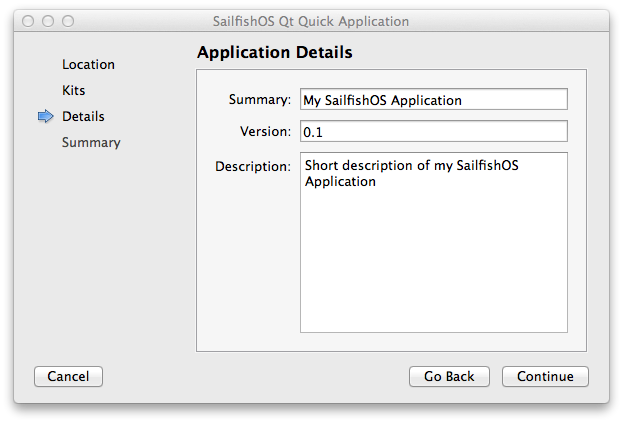
\includegraphics[scale=0.45]{../media/gfx/QtCreator/newsailfishproject05.png} 
  \caption{First example, step 5.}
  \label{fig:newsailfishproject05}
\end{figure}
%
%
\begin{figure}[H]
  \centering
  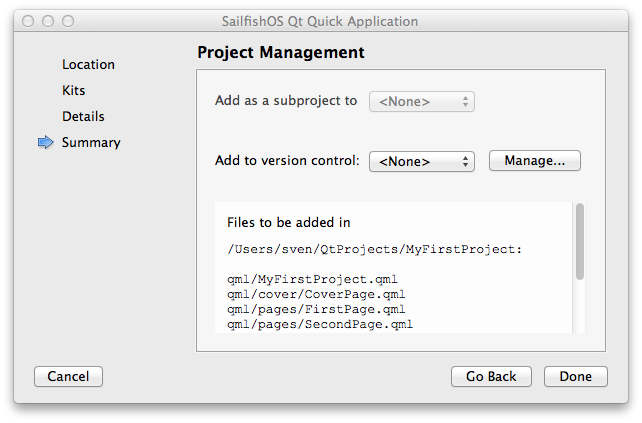
\includegraphics[scale=0.45]{../media/gfx/QtCreator/newsailfishproject06.png} 
  \caption{First example, step 1.}
  \label{fig:newsailfishproject06}
\end{figure}
%

Start the SDK from inside the QtCreator.
\begin{figure}[H]
  \centering
  
\includegraphics[scale=1.0]{../media/gfx/QtCreator/SDKstart.png} 
  \caption{Starting the SDK.}
  \label{fig:sdkstartcreator}
\end{figure}
%
When the virtual machine with the SDK is running, apply updates if necessary. %
\begin{figure}[H]
  \centering
  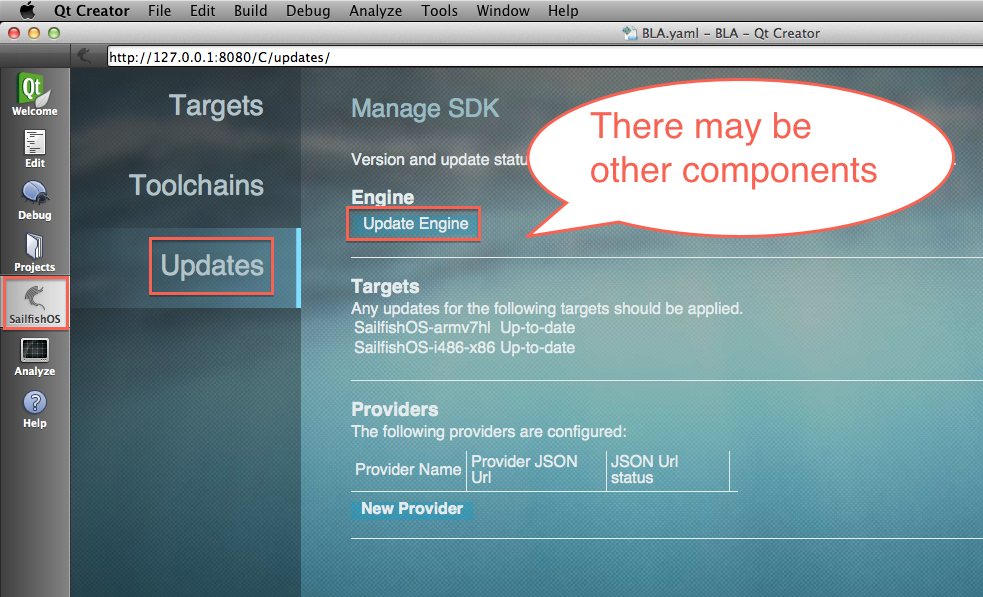
\includegraphics[scale=0.4]{../media/gfx/QtCreator/managesdkupdate.png} 
  \caption{Updating the SDK.}
  \label{fig:managesdkupdate}
\end{figure}
%
Start the Emulator.
\begin{figure}[H]
  \centering
  
\includegraphics[scale=1.0]{../media/gfx/QtCreator/SDKemulator.png} 
  \caption{Starting the Emulator.}
  \label{fig:emulatorstartcreator}
\end{figure}
%
Compile and run your application.
\begin{figure}[H]
  \centering
  
\includegraphics[scale=1.0]{../media/gfx/QtCreator/runappincreator.png} 
  \caption{Build and run the application.}
  \label{fig:runappincreator}
\end{figure}
%
Easy as pie, also see figure \ref{fig:emulatorexample} on page \pageref{fig:emulatorexample}. But what happens when and where if you click on those Icons? Look in section \textit{\nameref{sec:tools}}.

A good starting point to look for a more sophisticated starting example is \emph{The missing HelloWorld. Wizard included} by Artem Marchenko\cite{gh01}. You should check that out! It has all the tweaks needed to bring your app to the Jolla store!

And you should look in the \verb,examples, folder of the SDK of course.
%